\documentclass[12pt]{article}
\usepackage[russian]{babel}
\usepackage{geometry}

%библиотеки для задания 2
\usepackage{graphicx}
\usepackage{caption}

\usepackage{enumitem}

\usepackage{verbatim}

%нестандартные математические обозначения
\usepackage{amssymb}
\usepackage{amsmath}

%различные цветовые модели
\usepackage[usenames]{color}
\usepackage[dvipsnames,table]{xcolor}
\usepackage{colortbl}

\usepackage{listings}
\usepackage{listingsutf8}
\usepackage[T2A]{fontenc}
\newcommand{\listingsttfamily}{\usefont{T2A}{PTMono-TLF}{m}{n}}

\lstset{
	language=C,                % choose the language of the code
	numbers=left,                   % where to put the line-numbers
	stepnumber=1,                   % the step between two line-numbers.        
	numbersep=5pt,                  % how far the line-numbers are from the code
	backgroundcolor=\color{black},  % choose the background color. You must add \usepackage{color}
	commentstyle=\color{Gray},
	basicstyle=\listingsttfamily\color{Gray},
	keywordstyle=\color{BurntOrange},
	stringstyle=\color{YellowGreen},
	showspaces=false,               % show spaces adding particular underscores
	showstringspaces=false,         % underline spaces within strings
	showtabs=false,                 % show tabs within strings adding particular underscores
	tabsize=4,                      % sets default tabsize to 2 spaces
	captionpos=b,                   % sets the caption-position to bottom
	breaklines=true,                % sets automatic line breaking
	breakatwhitespace=true,         % sets if automatic breaks should only happen at whitespace
	title=\lstname, 
	inputencoding=utf8,                % show the filename of files included with \lstinputlisting;
	extendedchars=\true,
	keepspaces=true
}

%параметры документа
\geometry{top=2cm, bottom=2cm, left=1cm, right=1cm}
\textheight=24cm
\textwidth=18cm
\flushbottom 

\oddsidemargin=0pt 
\topmargin=-1.5cm 
\parskip=0pt
\parindent=24pt 

\tolerance=2000 

\begin{document}
	\begin{center}
		{\parskip=1cm
			МИНИСТЕРСТВО НАУКИ И ВЫСШЕГО ОБРАЗОВАНИЯ РОССИЙСКОЙ ФЕДЕРАЦИИ
			
			ФЕДЕРАЛЬНОЕ ГОСУДАРСТВЕННОЕ БЮДЖЕТНОЕ ОБРАЗОВАТЕЛЬНОЕ УЧРЕЖДЕНИЕ ВЫСШЕГО ОБРАЗОВАНИЯ
			
			{\bf«БЕЛГОРОДСКИЙ ГОСУДАРСТВЕННЫЙ ТЕХНОЛОГИЧЕСКИЙ УНИВЕРСИТЕТ им. В. Г. Шухова»\\(БГТУ им. В. Г. Шухова)}
			
		
			Кафедра программного обеспечения вычислительной техники и автоматизированных систем
		}
		
		\vspace{5cm}
		
		{\Large 
			{\bf
				 Лабораторная работа №8
				
				курса <<Алгоритмы и структуры данных>>
				
			}
			
		}
	\end{center}
	\begin{flushright}
		{\parskip=3cm Выполнил студент}
		
		Пугачев Вячеслав Эдуардович
		
		Группа: КБ-231
		
		Проверил:
		
		Акиньшин Даниил Иванович
	\end{flushright}
	\begin{center}
		{\parskip=3cm Белгород, 2024}
	\end{center}
	\newpage
	
	{\bf Цель работы:} изучить СД типа <<таблица>>, научиться их программно реализовывать и использовать.
	
	{\bf Задания:}
	
	\setlist[3]{noitemsep} % sets the itemsep and parsep for all level two lists to 0
	
	\begin{enumerate}
	
	\item Для СД типа <<таблица>> определить:
	
		\begin{enumerate}
	
			\item Абстрактный уровень представления СД:
			
			\begin{enumerate}
	
				\item Характер организованности и изменчивости, 
	
				\item Набор допустимых операций.
			
			\end{enumerate}
	
			\item Физический уровень представления СД:
			
			\begin{enumerate}
	
				\item Схему хранения;
	
				\item Объем памяти, занимаемый экземпляром СД;
	
				\item Формат внутреннего представления СД и способ его  интерпретации;
				
				\item Характеристику допустимых значений;
				
				\item Тип доступа к элементам.
				
			\end{enumerate}
			
			\item Логический уровень представления СД. Способ описания СД и экземпляра СД на языке программирования.
	
		\end{enumerate}
	
	\item Реализовать СД типа <<таблица>> в соответствии с вариантом индивидуального задания в виде модуля;
	
	\item Разработать программу для решения задачи в соответствии с вариантом индивидуального задания с использованием модуля, полученного в результате выполнения пункта 2 задания.
	
	\end{enumerate}
	
	\setcounter{secnumdepth}{-1} 
	\tableofcontents
	\newpage
	
	{\parskip=0.15cm
	
	\section{Задание 1:}
	\label{task_1}
	
	\subsection{Абстрактный уровень:}
	\label{task_1_1}
	\subsubsection{Задание 1.1.1:}
	\label{task_1_1_1}
	
	СД типа <<таблица>> --- еще одна СД в ряду нелинейных структур. Также она не является и иерархической. Она представляет собой множество пар $<K, V>$, где $K$ --- ключ текущей пары, а $V$ --- ее значение. Все пары в таблице имеют одинаковую организацию, то есть как ключи, так и значения имеют некоторый общий формат и тип. Все ключи в таблице обязательно уникальны: они и используются для идентификации и доступа к элементам при работе с таблицами --- в то время как значения могут повторяться. Конечно, для типа значения, используемого для ключей (число или строка), чаще всего определена операция сравнения, и ключи можно упорядочить (что иногда и делается в целях ускорения поиска по ключам путем применения алгоритма бинарного поиска). Но на абстрактном уровне пары <<ключ-значение>> все же не всегда можно назвать упорядоченными: между элементами может не существовать смысловой последовательной связи. Скорее, таблица представляет собой пары <<идентификатор объекта --- описание некоторых его свойств>>, в то время как сами объекты могут быть между собой не связаны. Поэтому таблица и относится к особому, табличному типу СД. 
	
	<<Таблица>> является динамической СД: пары <<ключ-значение>> в ходе работы могут добавляться и удаляться, а также могут перезаписываться значения по некоторому ключу.
	
	\subsubsection{Задание 1.1.2:}
	\label{task_1_1_2}
	Для СД типа <<таблица>> определены следующие операции, обязательные для любого варианта реализации этой структуры:
	
	\begin{enumerate}
	\item Инициализация,
	\item Включение элемента,
	\item Исключение элемента с заданным ключом,
	\item Чтение элемента с заданным ключом,
	\item Изменение элемента с заданным ключом,
	\item Проверка пустоты таблицы,
	\item Уничтожение таблицы
	\end{enumerate}
	
	\subsection{Физический уровень:}
	\label{task_1_2}
	\subsubsection{Задание 1.2.1:}
	\label{task_1_2_1}
	Для хранения СД типа <<таблица>> может использоваться как последовательная, так и связная схема хранения --- в зависимости от того, какая вспомогательная СД была выбрана для реализации. Если элементы включаются и исключаются без сохранения упорядоченности ключей в этой вспомогательной структуре, то используется последовательный или односвязный линейный список. Если упорядоченность сохраняется (для использования потом в поиске), то может использоваться как последовательный или односвязный список, так и бинарное дерево. Если же реализуется хэш-таблица, то есть  множество возможных ключей $K$ переводится в множество возможных адресов $A$ с помощью некоторой хэш-функции $H(k) = a$, то для хранения элементов обычно выбирается массив.
	
	Для реализации на ПЛС схема хранения последовательная, для массива в хэш-таблицах --- последовательная с некоторыми оговорками (см. задание 1.2.3), для реализации на ОЛС или бинарном дереве --- связная.
	
	\subsubsection{Задание 1.2.2:}
	\label{task_1_2_2}
	Количество памяти, занимаемой СД типа <<таблица>>, зависит от того, какое количество памяти занимает его ключ и базовый тип, выбрана ли последовательная или связная схема хранения (нужно ли отводить место для хранения указателей), сколько пар <<ключ-значение>> содержит таблица. Пусть базовый тип занимает $T$ байт, ключ --- $S$ байт, таблица содержит $K$ пар. Если таблица хранится на массиве или последовательном линейном списке (соответственно, дополнительная информация о паре не хранится), то количество памяти, занимаемой экземпляром СД <<дерево>>, будет равно $(T+S)*K$ байт. Если таблица хранится на односвязном линейном списке, то каждую пару необходимо сопровождать указателем на следующую; один указатель типа unsigned long занимает 8 байт, и вся таблица будет занимать $(T+S+8)*K$ байт. Если таблица хранится на бинарном дереве, то каждая пара будет сопровождаться двумя указателями, на левое и правое поддерево, и вся таблица будет занимать $(T+S+16)*K$ байт. Наконец, если мы говорим о хэш-таблице, то хранить ключи пар необязательно: на ключ уже указывает адрес, по которому хранится таблица. Значит, таблица будет занимать $T*K$ байт.
	
	\subsubsection{Задание 1.2.3:}
	\label{task_1_2_3}
 	Формат внутреннего представления СД <<таблица>> также зависит от выбора вспомогательной структуры для реализации. Если таблица реализуется на ПЛС, то двоичные коды элементов (правило перевода ключей и значений в двоичный код диктуется типом ключа и значения) хранятся последовательно друг за другом. В случае с хэш-таблицами двоичные коды значений таблицы хранятся в массиве, но уже не друг за другом; они разъединены пустыми пространствами, зарезервированными для хранения значений по ключам, которые на данный момент в таблицу не включены. Если таблица реализуется на ОЛС или бинарном дереве, то каждая пара <<ключ-значение>> включается в структуру <<запись>> с одним (для ОЛС) или двумя (для бинарного дерева) указателями на следующий или на дочерние элементы. Тогда элементы хранятся в памяти компьютера независимо друг от друга, а поля структуры <<запись>> также могут храниться не подряд или в отличном от заданного порядке. Указатели кодируются как беззнаковые целые числа --- пеерводятся в двоичную систему счисления и дополняются нулями слева до 64 разрядов (размера в 8 байт).

	\subsubsection{Задание 1.2.4:}
	\label{task_1_2_4}
	
	Количество и диапазон допустимых значений для СД типа <<таблица>> определяется количеством и диапазоном допустимых значений ее базового типа (типа значений в парах <<ключ-значение>>). Если таблица имеет фиксированное количество $K$ пар <<ключ-значение>>, то при расчете кардинального числа не учитывается диапазон значений ключей. Условно говоря, считается, что определен некоторый неизменный набор из $K$ ключей, для которых выбираются значения, причем таблицы считаются разными, если в них один и тот же набор значений по-разному распределен между ключами. Тогда для каждого из $K$ ключей выбирается значение из множества допустимых значений мощностью $CAR(BaseType)$, и кардинальное число для такой таблицы будет равно $CAR(BaseType)^K$. Кардинальное число СД <<таблица>> в целом определяется в конечном итоге как сумма по всем возможным значениям количества пар $CAR(Table) = \sum_{i = 0}^{max}{CAR(BaseType)^i}$, где $max$ --- максимальное количество элементов (определяется объемом памяти, отведенным для хранения таблицы). 
		
	\subsubsection{Задание 1.2.5:}
	\label{task_1_2_5}
	Тип доступа к элементам СД типа <<таблица>> зависит от того, является ли таблица неупорядоченной, упорядоченной или хэш-таблицей. В неупорядоченных таблицах пары <<ключ-значение>> хранятся вне зависимости от значения ключа; для поиска нужного элемента применяется линейный поиск, и нужно перебрать все элементы, хранящиеся перед искомым. В упорядоченных таблицах пары хранятся по возрастанию/убыванию ключей, и для поиска элемента с нужным ключом в таких таблицах может применяться бинарный поиск или поиск по дереву --- однако такой доступ также относится к последовательным. А вот в хэш-таблицах от ключа зависит, в какую область памяти будет записана пара <<ключ-значение>>. Потому, зная ключ, можно напрямую обратиться к этой области памяти --- для таких таблиц доступ будет прямым.
	
	\subsection{Логический уровень:}
	\label{task_1_3}
	СД типа <<таблица>> является производной СД, и описать ее на логическом уровне (представить на языке программирования) можно только после  самостоятельной ее реализации тем или иным способом. Приведем здесь описания для той реализации, которая будет выполнена в задании 2 этой лабораторной работы (неупорядоченная таблица на односвязном линейном списке).
	
	\lstinputlisting{../АСД 8 си/Table/Table_example.c}
	
	Однако для такой таблицы определен только тип ключа, но не задано ничего более --- ни тип базового элемента, ни его размер, ни одна из пар <<ключ-значение>> для этой таблицы. Все это будет возможно после написания модуля для работы с таблицами. 
	
	
	\begin{center}
	{\bf Индивидуальное задание; вариант 21}
	\end{center}
	{\bf Модуль 2:} Неупорядоченная таблица на односвязном линейном списке.
	
	Реализация на языке C:
	
	{\it \#if !defined(\_\_TABLE1\_H)
	
	\#define \_\_TABLE1\_H
	
	\#include "list3.h" // Cмотреть лаб.раб. №5
	
	const TableOk = 0;
	
	const TableNotMem = 1;
	
	const TableUnder = 2;
	
	typedef List Table;
	
	typedef ... T\_Key; // Определить тип ключа
	
	typedef int (* func)(void*, void*); /* Сравнивает ключи элементов таблицы, адреса которых находятся в параметрах a и b. Возвращает –1, если ключ элемента по адресу a меньше ключа элемента по адресу b, 0 — если ключи равны и +1 — если ключ элемента по адресу a больше ключа элемента по адресу b */
	
	int TableError; // 0..2
	
	void InitTable(Table *T, unsigned SizeMem, unsigned SizeEl); 
	inline int EmptyTable(Table *T); /* Возвращает 1 , если таблица пуста, иначе — 0 */
	
	int PutTable(Table *T, void *E, func f); /* Включение элемента в таблицу. Возвращает 1 , если элемент включен в таблицу, иначе — 0 (если в таблице уже есть элемент с заданным ключем или нехватает памяти) */
	
	int GetTable(Table *T, void *E,  T\_Key Key, func f);  /* Исключение элемента. Возвращает 1 , если элемент с ключем Key  был в таблице, иначе — 0 */
	
	int ReadTable(Table *T, void *E, T\_Key Key, func f); /* Чтение элемента. Возвращает 1 , если элемент с ключем Key есть в таблице, иначе — 0 */
	
	int WriteTable(Table *T, void *E, T\_Key Key, func f);  /* Изменение элемента. Возвращает 1 , если элемент с ключем Key есть в таблице, иначе — 0 */
	
	void DoneTable(Table *T); //Удаление таблицы из динамической памяти 
	
	\#endif}
	
	{\bf Задача 3:} Текст программы на некотором алгоритмическом языке может содержать символы-разделители, служебные слова, числовые константы и идентификаторы (слова, начинающиеся не с цифры и не являющиеся служебными). Проверить ошибки в записи идентификаторов и констант, парность служебных слов: <<BEGIN>> и <<END>>, <<IF>> и <<THEN>>, <<FOR>> и <<DO>>, и скобок: <<(>> и <<)>>, <<[>> и <<]>>. Проверку констант выполнить с помощью стандартной процедуры VAL. Для проверки парности служебных слов и символов-разделителей использовать динамический массив из KP целочисленных элементов, где KP — количество парных служебных слов и символов-разделителей. Сначала все элементы массива обнуляются. Если встречается первое слово i-й пары, то i-й элемент массива увеличивается на единицу, а если второе слово — уменьшается. После обработки текста программы все элементы массива должны быть нулевыми. Парные служебные слова  и  символы-разделители  хранить  в  таблице.  Ключ  элемента  таблицы — парное служебное слово, информационная часть содержит +i для первого слова i-й пары и –i для второго слова. Информацию о символах-разделителях и парных служебных словах прочитать из текстовых файлов.
	
	\section{Задание 2:}
	\label{task_2}
	
	Если перед нами стоит задача реализовать неупорядоченную таблицу на односвязном линейном списке, необходимо сначала реализовать сам односвязный линейный список. В рамках лабораторной работы №5 мы реализовывали односвязный линейный список, однако он имел базовый типа int, а в нашем случае базовым типом должен быть пустой указатель, что требует изменения кода некоторых функций. Таким образом, реализуем сначала модуль для работы с односвязными линейными списками.
	
	Не будем углубляться в объяснения, поскольку, как уже было сказано, похожий код мы уже писали в рамках работы №5. Следующим образом будет выглядеть заголовочный файл:
	
	\lstinputlisting{../АСД 8 си/VoidSingleList/VoidSingleList.h}
	
	...А следующим --- файл реализации. 
	
	\lstinputlisting{../АСД 8 си/VoidSingleList/VoidSingleList.c} 
			
	Код модуля для таблиц также будет разделен на файлы заголовка и реализации. В заголовочном файле зададим константы с кодами двух основных ошибок, которые могут возникнуть в ходе работы с таблицами: TableNotMem --- не удалось выделить место под хранение нового элемента таблицы; TableUnder --- попытка прочесть элемент из пустой таблицы. Под хранение кода ошибки отводится переменная. 
	
	После этого дадим название используемым типам данных. СД <<таблица>> объявляется как переименование СД <<односвязный линейный список>>, у которого базовый тип --- пустой указатель. Затем объявляется тип ключа, T\_Key, как массив символов (строка) длиной 16; на практике же максимальная длина строки, которая может использоваться как ключ --- 15, а шестнадцатая позиция отводится под ноль-символ (такой тип ключа был выбран, опираясь на условия задания 3). Немного подкорректировав данный для варианта 21 шаблон, получим такой заголовочный файл:
	
	\lstinputlisting{../АСД 8 си/Table/Table.h} 
		
	Реализация функций будет вынесена в отдельный файл со следующим содержанием.
	
	{\bf Примечание: } будем считать базовым типом не самой таблицы, но списка, хранящего элементы таблицы, будем считать пустой указатель на область памяти, где хранятся последовательно ключ и значение пары. Причем ключ отделен от значения одним (если его длина достигает 15) или несколькими (если эта длина меньше) нуль-символами, чт позволяет нам сравнивать по ключу и два значения типа char[16], и ключ с парой <<ключ-значение>>, и две пары. При записи, извлечении, чтении и перезаписи значения будем считать, что включается, исключается, считывается и перезаписывается вся пара, представленная в вышеописанном формате, и как аргумент должен передаваться указатель на такую пару. Такой подход потребует от нас дополнительных функций, которые будут описаны позднее.
	
	На мысль о таком подходе наводит то, что прототип функции PutTable имеет аргумент типа пустой указатель, но не имеет аргумента типа T\_Key --- значит, пустой указатель должен одновременно хранить и ключ, и значение. Логично распространить такой подход и на остальные функции.
	
	\lstinputlisting{../АСД 8 си/Table/Table.c} 
	
	Примечательно, что в итоге сценарий чтения или извлечения из пустой таблицы не приводит к ошибке --- извлечение и чтение производится по ключу, и для программы равнозначны сценарии, когда ключ не найден в пустой или непустой таблице.

	Для нормальных (не вызывающих ошибки и аварийного завершения) сценариев этих функций можно составить автоматизированные тесты и вынести их в отдельный файл тестирования. Порядок функций при тестировании может быть немного изменен, поскольку для заполнения таблиц значениями необходима функция PutTable, ее следует отладить раньше. Для тестирования объявляется базовый тип таблицы --- целочисленный тип int.
	
	{\bf Примечание: } здесь также определяются как функция сравнения ключей, так и функции для записи по пустому указателю одновременно и ключа, и значения некоторой строки таблицы, и извлечения значения из нее. Последние две функции не могут быть объявлены ранее, потому что привязаны к базовому типу таблицы, который объявляется для каждого файла отдельно, а не в заголовочном файле модуля.
	
	\lstinputlisting{../АСД 8 си/Table/Table_test.c} 
		
	Запустив программу, можем самостоятельно убедиться, что все тесты прошли успешно:
	
	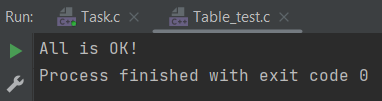
\includegraphics[width=120mm]{images/table_test_output.png} 
	
	\section{Задание 3:}
	\label{task_3}
	
	Теперь, когда модуль для СД типа <<таблица>> реализован, можем перейти к решению задачи для варианта 21, описанной выше. Как указано в условии, ключами таблицы, хранящей информацию о парных служебных словах и разделителях, должны быть сами эти слова, а значениями --- числа, отражающие номер пары; поэтому в качестве типа ключа мы оставляем строку не больше 15 символов, а в качестве значения --- целое число. 
	
	По сути, наша программа должна будет решать следующие подзадачи: 1) формировать таблицу для хранения информации о том, как служебные слова и разделители связаны в пары; 2) Создать пустой массив для хранения информации о том, сохраняется ли баланс открывающих и закрывающих слов для каждой пары, 3) Принимать имя файла, где записан текст кода, с клавиатуры, и записывать информацию из него в строку-буфер, 4) проходить по словам строки-буфера и для каждого делать выводы, является ли оно служебным словом или разделителем (и изменять массив <<баланса>> в таком случае), либо идентификатором, оператором или числовой константой, 5) по окончании обработки выводить информацию о найденных несоответствиях или ошибках или их отсутствии.
	
	Определим ряд вспомогательных функций. Для создания таблицы (и последующей с ней работы) нам понадобятся те же функции создания пары <<ключ-значение>> и извлечения значения из пары.
	
	\lstinputlisting[linerange={1-37}]{../АСД 8 си/Table/Table_test.c} 
	
	Для копирования информации из файла в буфер хватает стандартных функций библиотеки stdio. Для разделения строки  на слова воспользуемся набором функций из лабораторной работы №17 в рамках курса ОП (2-ой семестр). Точнее говоря, вводятся функции для поиска первого пробельного и непробельного символа, начиная с некоторого указателя. Объявляется также структура WordDescriptor, хранящая указатель на первый символ слова и символ, следующий за последним. Таким образом, можно ввести функцию, сохраняющую в структуру WordDescriptor указатели на начало и конец первого слова, встреченного после некоторого указателя. Также можно ввести функцию, перезаписывающую последовательность символов между указателями на начало и конец, в другую строку, со вставкой ноль-символа в конце.
	 
	\lstinputlisting[linerange={39-73}]{../АСД 8 си/Table/Task.c} 
	
	Когда задача разбиения строки на слова решена, можно ввести функцию, определяющую, является ли переданное ей слово ошибочно введенной переменной или числовой константой. Здесь требуются некоторые пояснения. Мы считаем словом последовательность символов, отделенную по краям пробельными символами, однако даже в языке программирования с самым лаконичным синтаксисом должны использоваться также операторы (обозначения арифметических операций, запятые), которые не всегда отделяются от идентификаторов и констант пробелами. Мы будем идти по переданному функции слову, задав изначально ложные флаги <<начато число>> и <<начат идентификатор>>. При считывании символа, если он является цифрой и флаг <<начат идентификатор>> является ложным, флаг <<начато число>> становится истинным. Если же был встречен символ алфавита или символ <<\_>>, при этом истинен флаг <<начато число>>, функция возвращает ложный результат; если же число не было начато, считается, что начат идентификатор. Если встреченный символ не является ни буквой, ни цифрой, проверяется, не относится ли он к списку <<запрещенных>>, то есть парных разделителей, зарезервированных для других целей. Если это не так, устанавливаются в значение false  флаги <<начато число>> и <<начат идентификатор>>; считается, что текущая последовательность символов рассмотрена, и далее идет некий оператор, отделяющий ее от следующей. ну а если встреченный символ все-таки относится к списку разделителей, функция возвращает false. 
	
	Получается, такая реализация требует, чтобы для корректной работы программы все парные разделители, как и парные служебные слова, были отделены пробелами и обособлены от остального кода.
	
	\lstinputlisting[linerange={75-105}]{../АСД 8 си/Table/Task.c} 
	
	Наконец, можно задать массив типа char как буфер перейти к телу функции main. Инициализируется таблица для хранения парных слов и разделителей, данные парные слова и разделители задаются в массиве литералов, и проходом по этому массиву формируются строки таблицы.
	
	Также инициализируется нулями массив для подсчета того, сколько раз встречались открывающие и закрывающие слова этих пар, и создается еще одна пустая таблица. Ее назначение поясним ниже.
	
	Затем запрашивается название файла с клавиатуры, файл связывается с файловой переменной, и его содержимое посимвольно копируется в буфер, пока не будет достигнут конец файла. После этого в буфере после содержимого файла добавляется нуль-символ, а файл закрывается.
	
	Далее вводится указатель для пробега по содержимому буфера, и запускается цикл, выполняющийся до тех пор, пока по этому указателю можно считать слово. В конце каждой итерации указатель сдвигается на позицию конца текущего слова. В теле же цикла содержимое слова копируется в отдельную строку, и первым делом проверяется: можно ли считать в заранее созданную переменную строку таблицы, если использовать текущее слово как ключ? Если можно, значит, найденное слово принадлежит к списку ключевых слов или разделителей. Из переменной, куда производилось копирование строки таблицы, считывается значение, по нему находится нужный индекс массива подсчета открывающих и закрывающих слов, и его значение увеличивается или уменьшается, в зависимости от того, положительно или отрицательно значение.
	
	Если считать строку таблицы по данному ключу нельзя, проверяется: является ли данное слово допустимой константой, переменной или их последовательностью, разделенной операторами? Если да, то никаких действий предпринимать не надо. Но если нет? Возможно, было бы логично просто вывести сообщение об ошибке и прекратить работу. С другой стороны, было бы удобно сразу получить как можно более полную информацию об имеющихся ошибках, а не перезапускать программу после каждого исправления имен переменных, только чтобы получить сообщение о новой ошибке. Но если выполнение программы будет продолжаться после найденной ошибки, а переменная с недопустимым именем используется снова и снова, то вывод будет состоять из множества однотипных сообщения. Значит, надо хранить информацию о том, какие недопустимые имена встречались и --- что тоже было бы полезно --- сколько раз. 
	
	Для этого нам и пригодится вторая таблица --- для хранения имен недоспустимых переменных. Если найденная последовательность признана ошибочной, конструируется переменная со строкой таблицы, где ключ --- данная последовательность, значение --- единица, и производится попытка прочитать строку по этому ключу в эту же переменную. Если она была успешной, значит, такая переменная уже встречалась: из строки считывается значение, конструируется новая строка, где это значение увеличивается на 1, и перезаписывается в таблицу. если же попытка чтения была неудачной, значит, такое ошибочное имя встречается впервые, и нужно занести строку в таблицу.
	
	В конце сначала производится проход по элементам массива-счетчика: если один из элементов не равен 0, то выводится сообщение, что соответствующая конструкция не завершена верно. Потом по очереди извлекаются строки из таблицы ошибочных имен, и выводится информация о том, какое из них сколько раз было встречено в программе. Если же ни одного вывода не было совершено, выводится сообщение о корректности программы.
	
	\lstinputlisting[linerange={107-179}]{../АСД 8 си/Table/Task.c} 
	
	Для того, чтобы протестировать полученную программу, будем использовать следующие демонстрационные тексты программ:
	
	\verbatiminput{../АСД 8 си/Table/task_test/data0.txt}
	
	В данном тексте программы ошибок нет, при этом используется несколько разных пар служебных слов, есть переменные, содержащие в своих именах цифры и символ <<\_>>, и переменные, соединенные операторами без пробелов.
	
	\verbatiminput{../АСД 8 си/Table/task_test/data1.txt}
	
	В данном тексте программы имена переменных не содержат ошибок, но есть ошибки в использовании парных служебных слов и разделителей: отсутствует закрывающая скобка <<[>> при наличии открывающей <<]>>, а также отсутствует служебное слово BEGIN, обозначающее начало блока для цикла FOR, тогда как END присутствует. 
		
	\verbatiminput{../АСД 8 си/Table/task_test/data2.txt}
	
	В данном тексте конструкции из парных слов не содержат ошибок, но есть ошибки в наименовании переменных: имя 1comp недопустимо по правилам именования. 
		
	\verbatiminput{../АСД 8 си/Table/task_test/data3.txt}
	
	В данном тексте есть как неправильно закрытые конструкции из парных слов (слово FOR не имеет парного ему слова DO), так и ошибки в именовании переменных: имя i( не будет правильно считываться, потому что название переменной не отделено от разделителя. 
	
	Запустим полученную программу для каждого из этих файлов:
	
	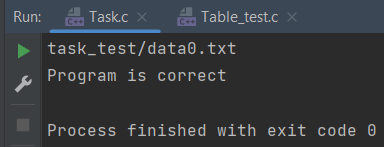
\includegraphics[width=70mm]{images/output0.png} 
	
	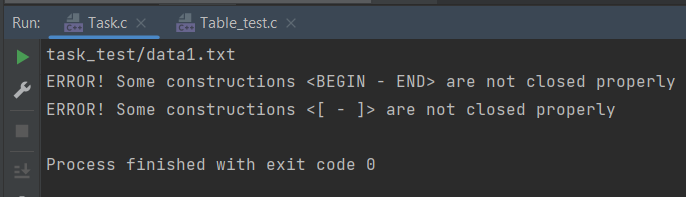
\includegraphics[width=110mm]{images/output1.png} 
	
	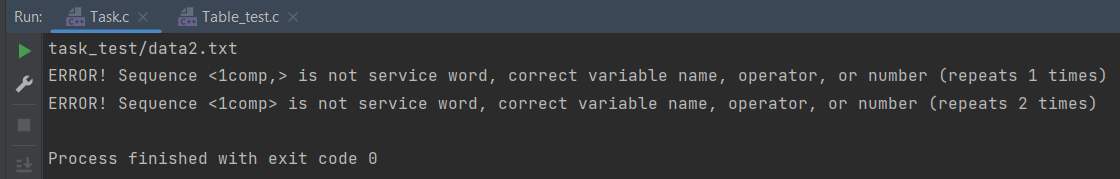
\includegraphics[width=180mm]{images/output2.png} 
	
	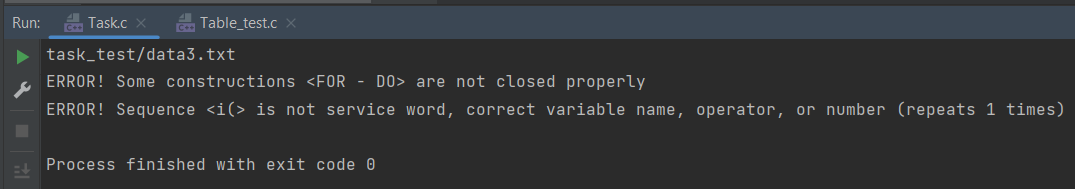
\includegraphics[width=180mm]{images/output3.png} 
	
	Легко заметить, что в конечном итоге вывод программы совпадает с нашими собственными размышлениями. 
	
	{\bf Примечание:} на примере обработки файла data2.txt, однако, видно, что хотя программа способна подсчитывать встреченные ошибочные последовательности, она не может отличить, является ли такая последовательность отдельным идентификатором или последовательностью из нескольких идентификаторов или операторов. Впрочем, по условию задачи этого и не требовалось.
	
	\section{Вывод:}
	
	В ходе лабораторной работы дали характеристику СД типа <<таблица>>, форматам ее представления, реализовали один из них в соответствии с вариантом (Неупорядоченная таблица на односвязном линейном списке с базовым типом <<пустой указатель>>), написали ряд базовых функций для работы с таблицами в этом формате, а также решили задачу проверки на синтаксические ошибки программы на алгоритмическом языке.
}
\end{document}